

\tikzset{every picture/.style={line width=0.75pt}} %set default line width to 0.75pt        

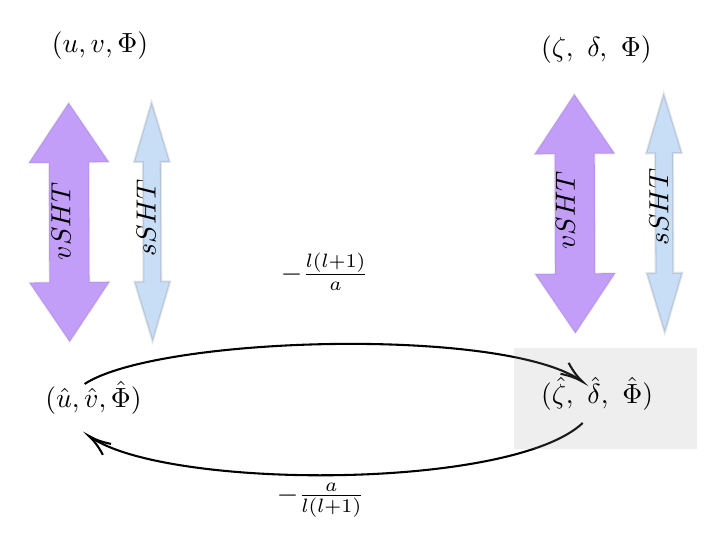
\begin{tikzpicture}[x=0.75pt,y=0.75pt,yscale=-1,xscale=1]
%uncomment if require: \path (0,300); %set diagram left start at 0, and has height of 300

%Left Right Arrow [id:dp2543051183422924] 
\draw  [color={rgb, 255:red, 0; green, 0; blue, 0 }  ,draw opacity=0.05 ][fill={rgb, 255:red, 194; green, 158; blue, 249 }  ,fill opacity=1 ] (162.91,50.1) -- (182.4,78.72) -- (172.72,78.82) -- (172.97,136.44) -- (182.65,136.34) -- (163.41,165.36) -- (143.92,136.74) -- (153.61,136.64) -- (153.35,79.02) -- (143.67,79.12) -- cycle ;
%Left Right Arrow [id:dp7369355028476874] 
\draw  [color={rgb, 255:red, 0; green, 0; blue, 0 }  ,draw opacity=0.1 ][fill={rgb, 255:red, 74; green, 144; blue, 226 }  ,fill opacity=0.3 ] (202.86,49.81) -- (211.59,78.54) -- (207.28,78.58) -- (207.54,136.21) -- (211.84,136.17) -- (203.36,165.07) -- (194.63,136.34) -- (198.93,136.3) -- (198.68,78.67) -- (194.38,78.72) -- cycle ;
%Left Right Arrow [id:dp47994436496181625] 
\draw  [color={rgb, 255:red, 0; green, 0; blue, 0 }  ,draw opacity=0.05 ][fill={rgb, 255:red, 194; green, 158; blue, 249 }  ,fill opacity=1 ] (406.55,45.95) -- (426.04,74.56) -- (416.36,74.66) -- (416.61,132.29) -- (426.3,132.19) -- (407.06,161.2) -- (387.57,132.59) -- (397.25,132.49) -- (397,74.86) -- (387.32,74.96) -- cycle ;
%Left Right Arrow [id:dp19367934898724093] 
\draw  [color={rgb, 255:red, 0; green, 0; blue, 0 }  ,draw opacity=0.1 ][fill={rgb, 255:red, 74; green, 144; blue, 226 }  ,fill opacity=0.3 ] (449.61,45.66) -- (458.34,74.38) -- (454.04,74.43) -- (454.29,132.05) -- (458.59,132.01) -- (450.12,160.91) -- (441.39,132.19) -- (445.69,132.14) -- (445.44,74.52) -- (441.14,74.56) -- cycle ;
%Curve Lines [id:da22359335462503038] 
\draw    (170.6,185.6) .. controls (205.88,162.56) and (371.38,157.93) .. (409.48,183.81) ;
\draw [shift={(410.6,184.6)}, rotate = 216.72] [color={rgb, 255:red, 0; green, 0; blue, 0 }  ][line width=0.75]    (10.93,-3.29) .. controls (6.95,-1.4) and (3.31,-0.3) .. (0,0) .. controls (3.31,0.3) and (6.95,1.4) .. (10.93,3.29)   ;
%Curve Lines [id:da8324860879521677] 
\draw    (410.6,204.4) .. controls (375.95,236.87) and (210.95,236.61) .. (173.69,211.37) ;
\draw [shift={(172.6,210.6)}, rotate = 36.61] [color={rgb, 255:red, 0; green, 0; blue, 0 }  ][line width=0.75]    (10.93,-3.29) .. controls (6.95,-1.4) and (3.31,-0.3) .. (0,0) .. controls (3.31,0.3) and (6.95,1.4) .. (10.93,3.29)   ;
%Shape: Rectangle [id:dp8400991491232823] 
\draw  [color={rgb, 255:red, 0; green, 0; blue, 0 }  ,draw opacity=0 ][fill={rgb, 255:red, 155; green, 155; blue, 155 }  ,fill opacity=0.17 ] (377.6,168.2) -- (465.6,168.2) -- (465.6,216.8) -- (377.6,216.8) -- cycle ;

% Text Node
\draw (153.28,14.44) node [anchor=north west][inner sep=0.75pt]    {$( u,v,\Phi )$};
% Text Node
\draw (150.17,182.86) node [anchor=north west][inner sep=0.75pt]    {$(\hat{u} ,\hat{v} ,\hat{\Phi })$};
% Text Node
\draw (389,16.52) node [anchor=north west][inner sep=0.75pt]    {$( \zeta ,\ \delta ,\ \Phi )$};
% Text Node
\draw (389,180.78) node [anchor=north west][inner sep=0.75pt]    {$(\hat{\zeta } ,\ \hat{\delta } ,\ \hat{\Phi })$};
% Text Node
\draw (263.69,121.04) node [anchor=north west][inner sep=0.75pt]    {$-\frac{l( l+1)}{a}$};
% Text Node
\draw (261.69,232.04) node [anchor=north west][inner sep=0.75pt]    {$-\frac{a}{l( l+1)}$};
% Text Node
\draw (153.21,127.51) node [anchor=north west][inner sep=0.75pt]  [rotate=-269.93]  {$vSHT$};
% Text Node
\draw (396.21,122.51) node [anchor=north west][inner sep=0.75pt]  [rotate=-269.93]  {$vSHT$};
% Text Node
\draw (194.21,125.51) node [anchor=north west][inner sep=0.75pt]  [rotate=-269.93]  {$sSHT$};
% Text Node
\draw (441.21,120.51) node [anchor=north west][inner sep=0.75pt]  [rotate=-269.93]  {$sSHT$};


\end{tikzpicture}
